\chapter{Case Study: Environment-aware Gradient Ascent}

A case study was conducted to demonstrate the capabilities of the proposed integration and to provide a practical starting point for users interested in experimenting with aggregate programming within Unity. Despite its conceptual simplicity, this case study encompasses the core challenges addressed in this thesis. The experiment was replicated across two distinct exemplars. The first utilizes a minimal environment optimized for logic verification and debugging, while the second employs a rich environment to demonstrate the potential of a modern game engine as a high-fidelity simulator.

\section{Case Study Statement}

The case study addresses a classic problem in the \ac{CAS} domain known as gradient ascent. In this scenario, a swarm of devices must navigate toward a source of interest while dynamically avoiding obstacles. The behavior is governed by two main logic streams involving collective intelligence and local obstacle avoidance. In the collective intelligence stream, devices sense the intensity of the source at their current location and share this data with their neighbors. By comparing local intensities, they collaboratively determine the direction of the steepest gradient, allowing the swarm to move toward the local best position. Simultaneously, each node perceives physical obstacles in its immediate vicinity. Unlike the source intensity, obstacle data is not shared between nodes; instead, each device independently adjusts its trajectory to maintain a safe distance from collisions.

All nodes execute synchronous rounds at a fixed frequency of $20Hz$. In each round, a node performs a sense-compute-act cycle. During the perception phase, it measures the local intensity of the source, which is calculated based on Euclidean distance and detects nearby obstacles or fellow agents. Communication and vicinities are established using a distance-based neighborhood model where two nodes are considered neighbors if their separation is within 10 units, forming the connectivity graph required for aggregate computation. During the computation phase, nodes exchange intensity data to compute a movement vector. This vector is the result of a weighted sum where one component points toward higher source intensity and another points away from obstacles. These gradient computations are performed using the Collektive standard library, which implements the foundational aggregate programming building blocks defined in the field's literature~\cite{DBLP:journals/tomacs/ViroliABDP18}.

\section{Minimal Environment}

The minimal scene consists of a simplified arena containing four parallelepipedic obstacles measuring 1x3x5 units that physically obstruct the path to the source. The devices are represented by spheres moving across a flat plane toward a source located at a fixed coordinate. This environment served as the primary benchmark for performance testing. On hardware with integrated graphics, the simulation maintained real-time performance with up to 50 nodes. On a desktop equipped with a dedicated GPU (NVIDIA RTX 4070), the system scaled easily to 100 nodes while maintaining a high frame rate. The progression of the swarm through this environment is illustrated in the snapshots in~\cref{fig:minimal-env}.

\begin{figure}
    \centering
    \includegraphics[width=.49\textwidth]{figures/min-env-1.png}
    \includegraphics[width=.49\textwidth]{figures/min-env-2.png}
    \includegraphics[width=.49\textwidth]{figures/min-env-3.png}
    \includegraphics[width=.49\textwidth]{figures/min-env-4.png}
    \caption{Screenshots of the minimal environment scenario with 100 nodes.}\label{fig:minimal-env}
\end{figure}

\section{Rich Environment}

To showcase the high-fidelity potential of the Unity integration, the experiment was replicated in a complex built-in environment titled `Oasis'. In this version, the abstract obstacles are replaced by complex geometries including trees, bushes, and rocks. The source of interest is placed inside a tent on the far side of the arena, requiring the nodes to navigate sophisticated terrain from their initial spawn point. The increased complexity of this environment, specifically regarding the detailed rendering, high-poly mesh collisions, and advanced physics interactions, significantly raised the computational requirements compared to the minimal scenario.

While a dedicated GPU is recommended to maintain optimal real-time performance, tests showed that an integrated GPU could still execute the simulation with a reduced load of 50 nodes, albeit reaching the limits of its processing capabilities. With a dedicated desktop GPU, the simulation comfortably handled 100 nodes, successfully demonstrating the swarm's ability to navigate natural obstacles while maintaining the aggregate gradient ascent logic. The evolution of the system in this rich environment is captured in~\cref{fig:rich-env}.

\begin{figure}
    \centering
    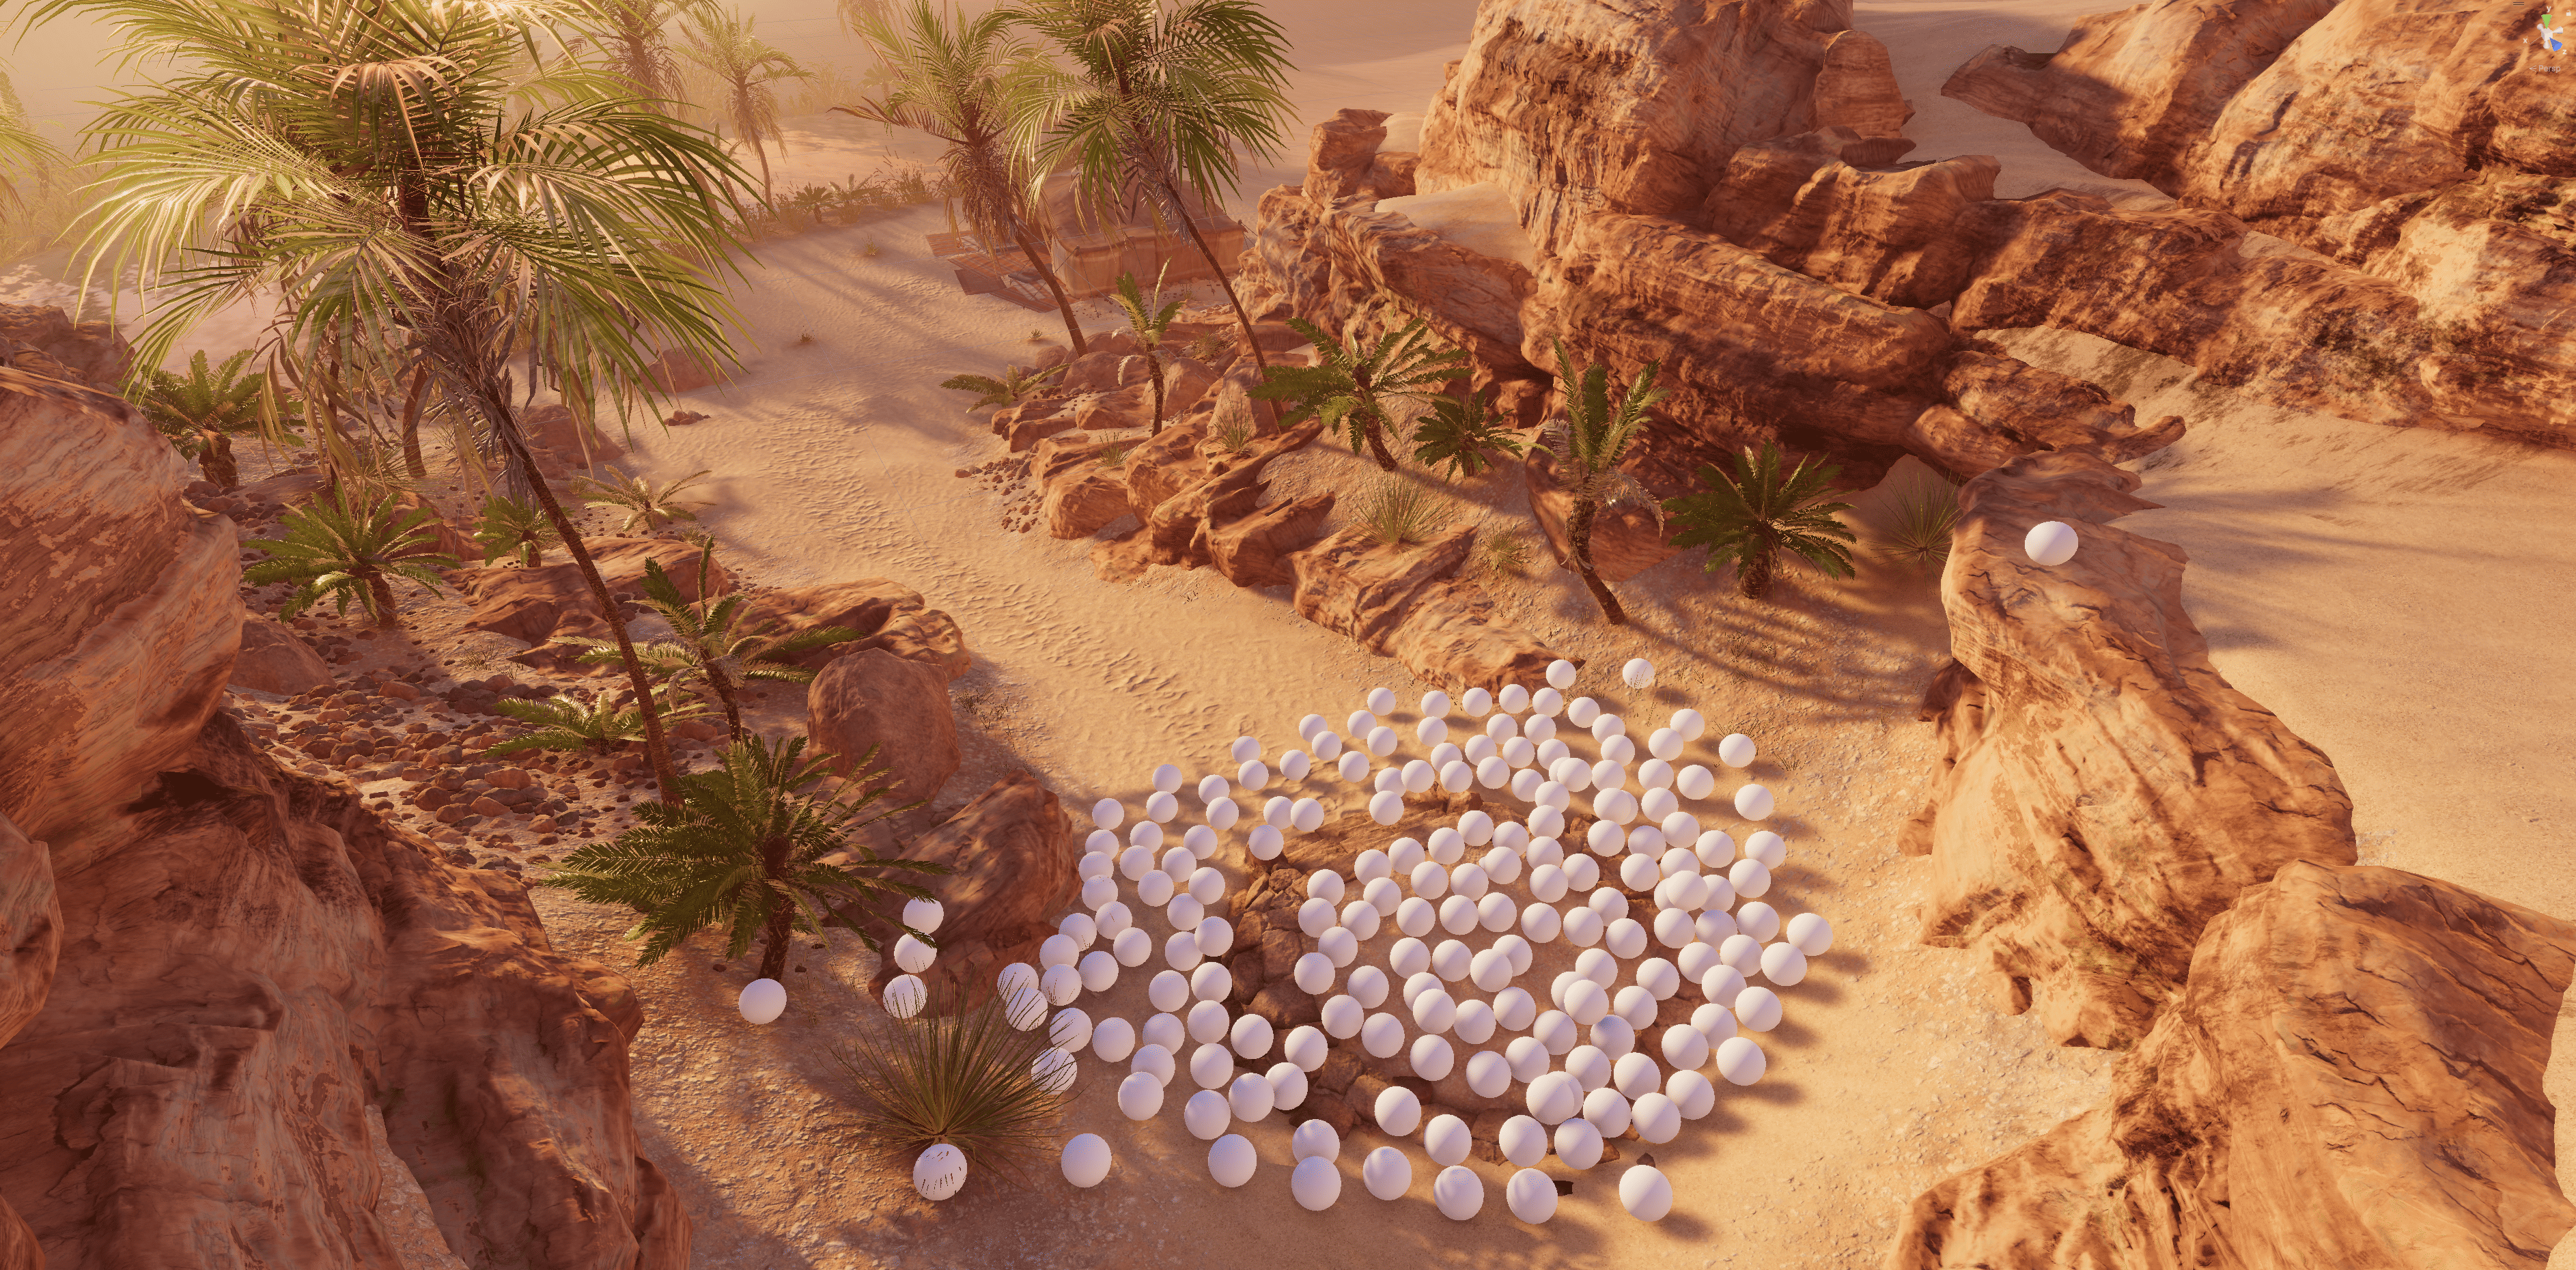
\includegraphics[width=.49\textwidth]{figures/rich-env-2.png}
    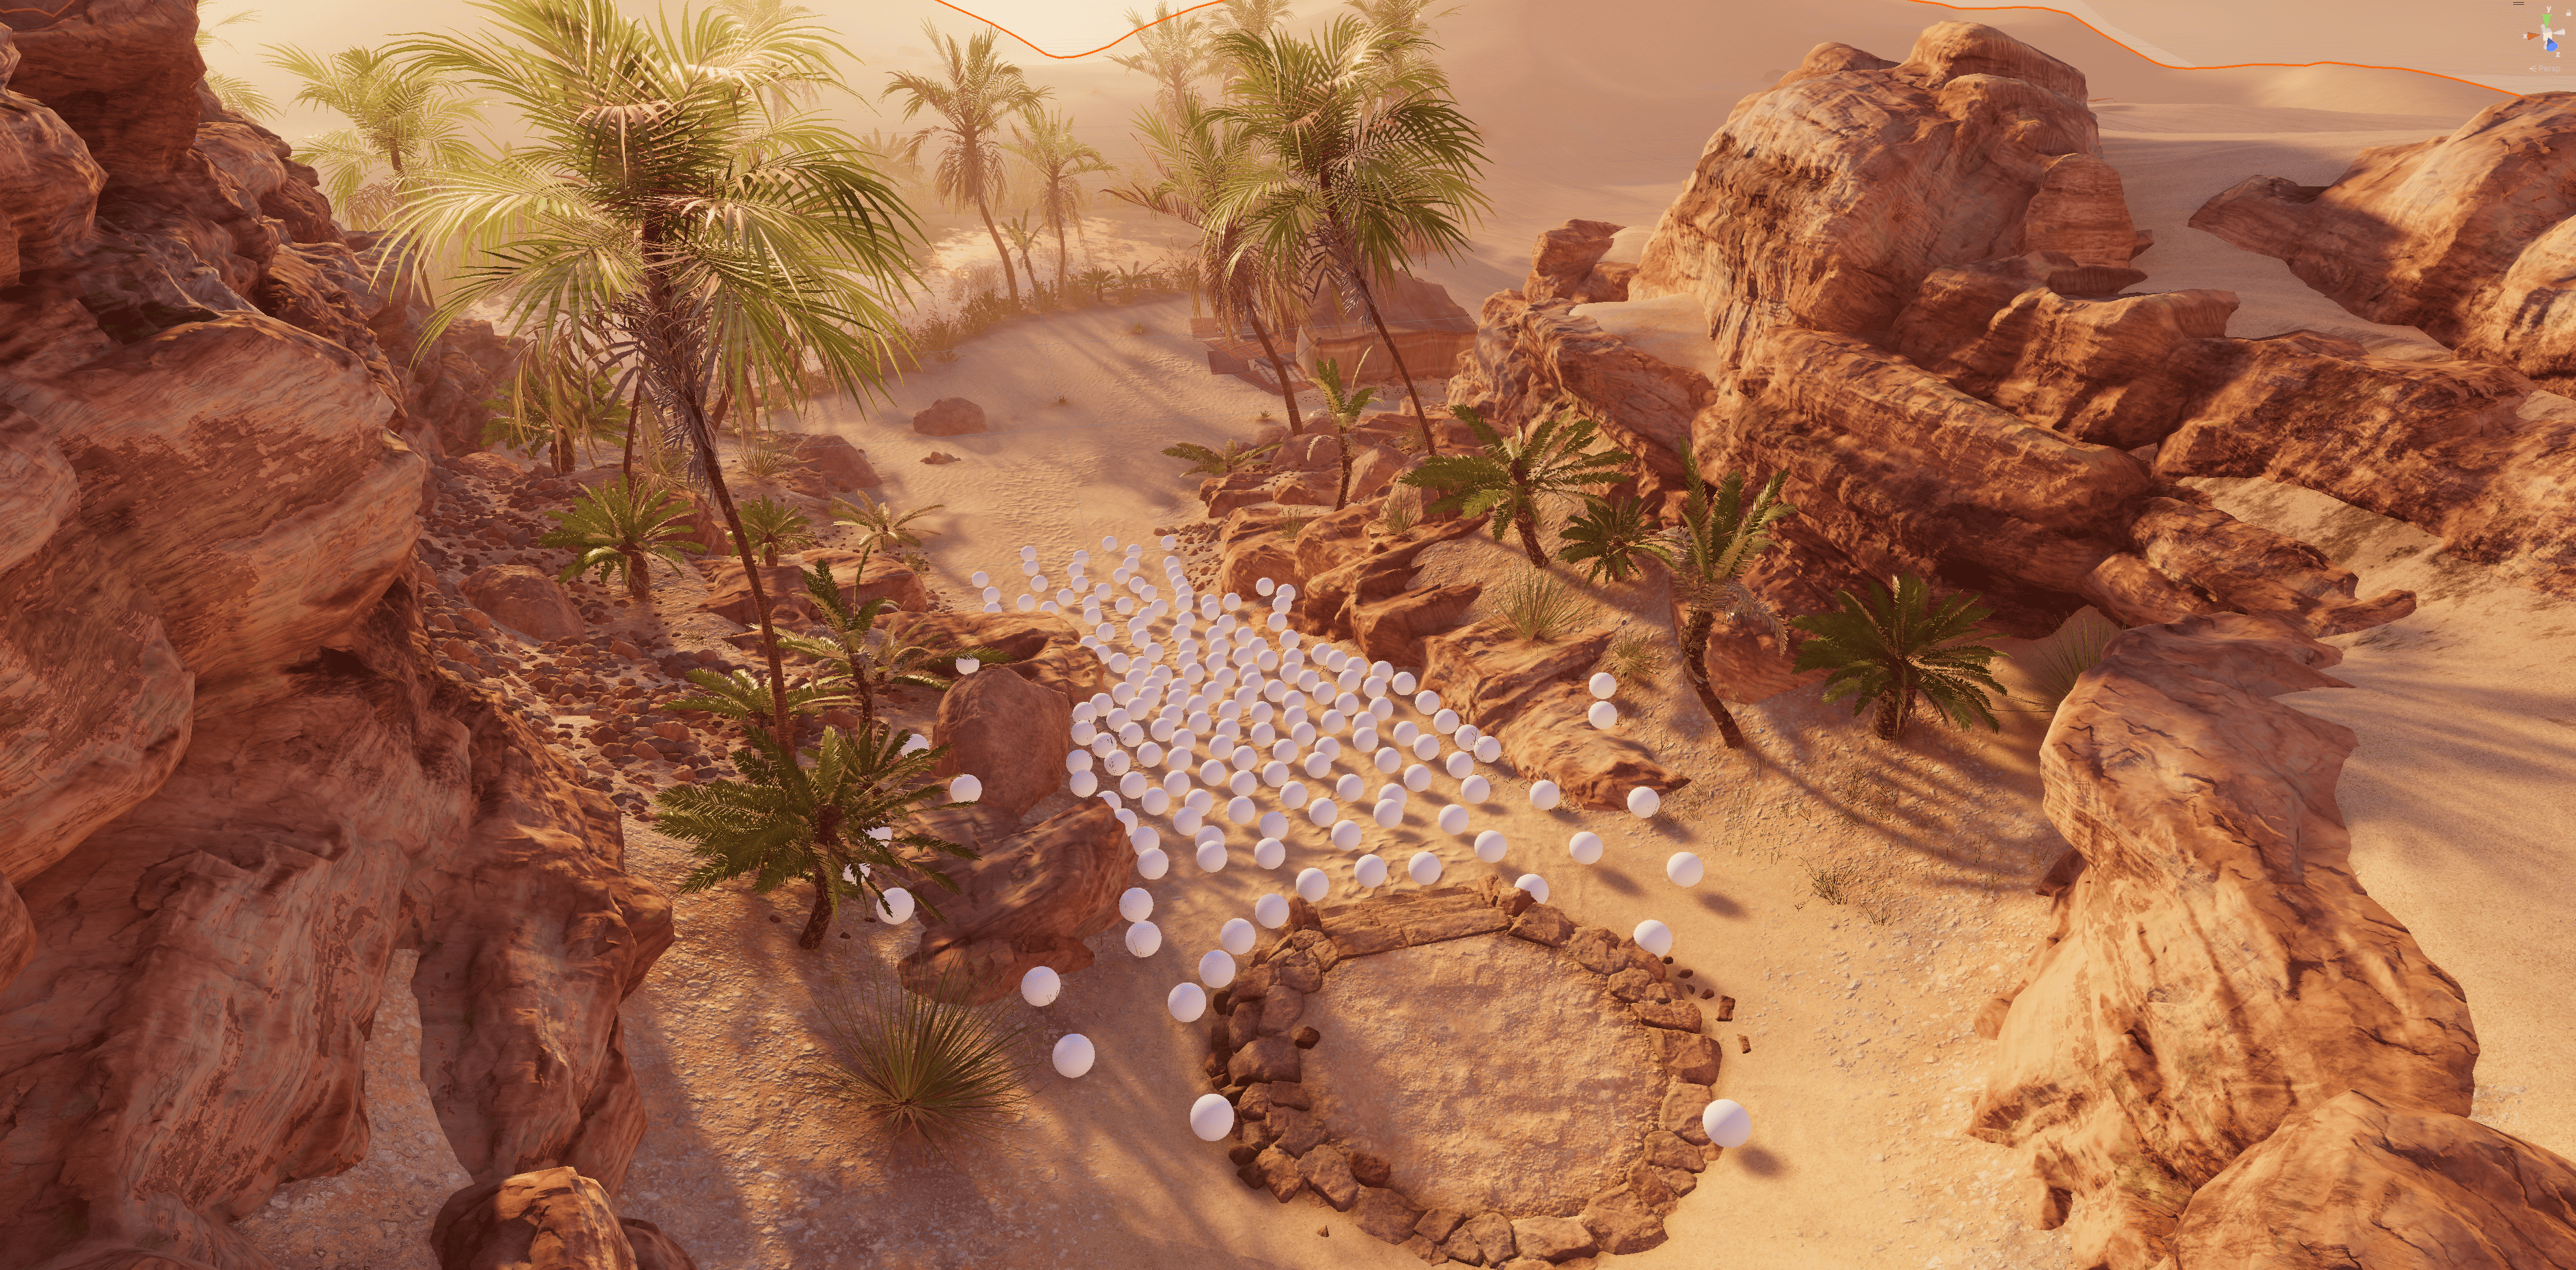
\includegraphics[width=.49\textwidth]{figures/rich-env-3.png}
    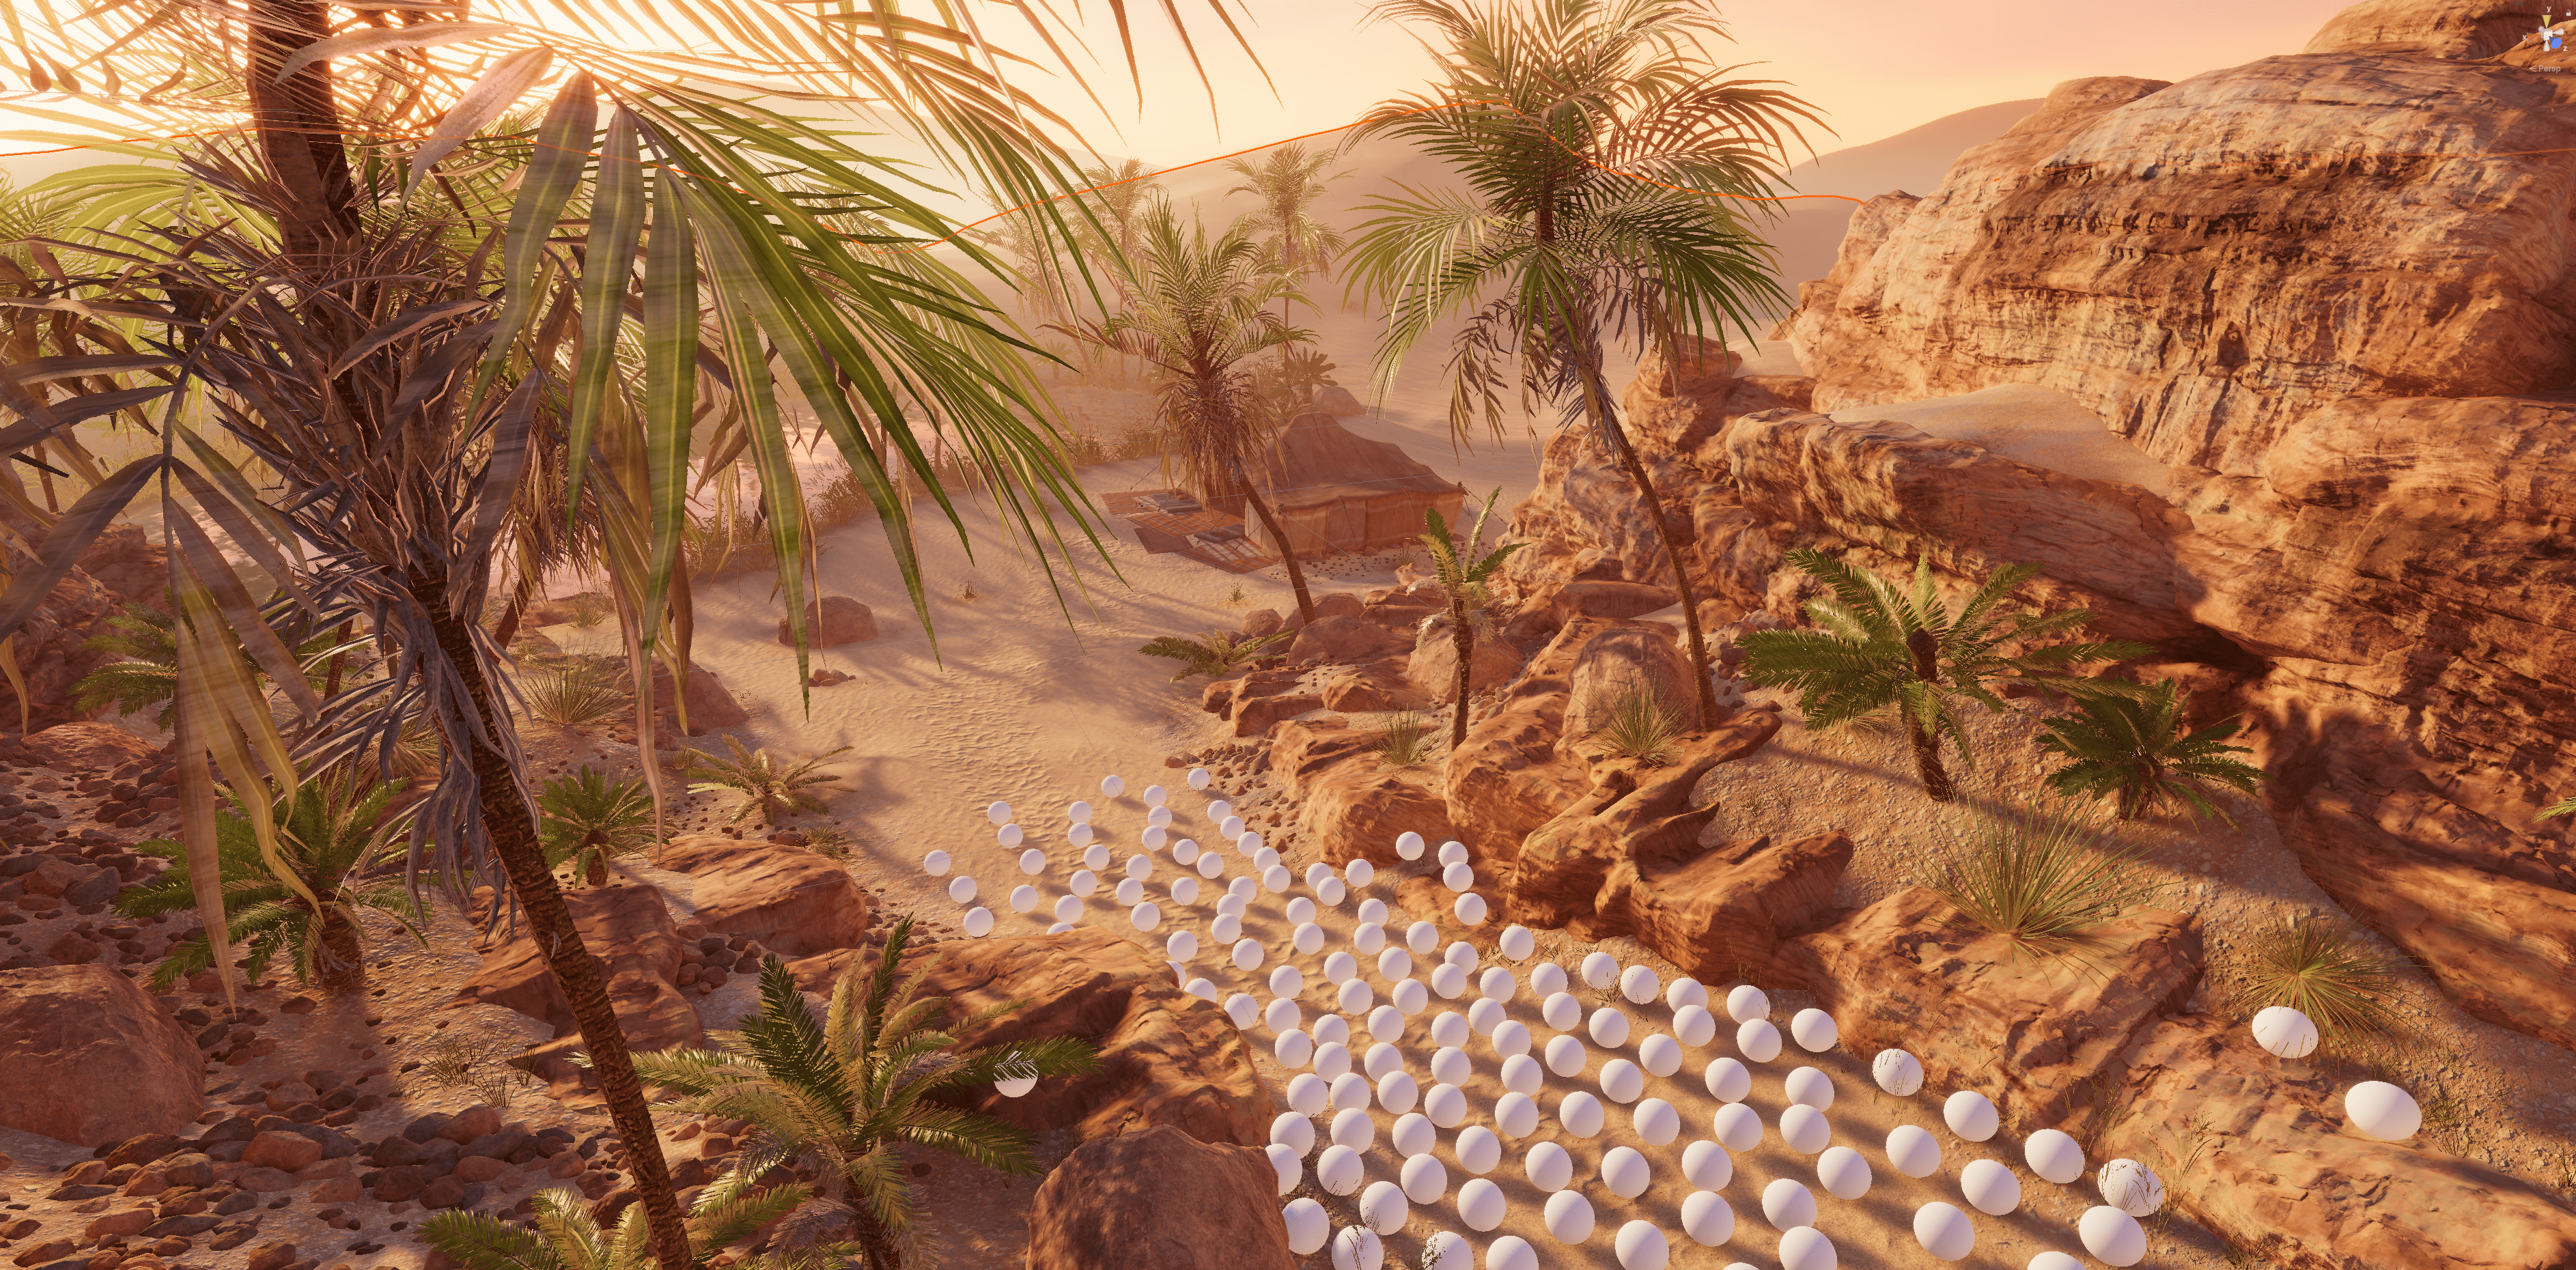
\includegraphics[width=.49\textwidth]{figures/rich-env-4.png}
    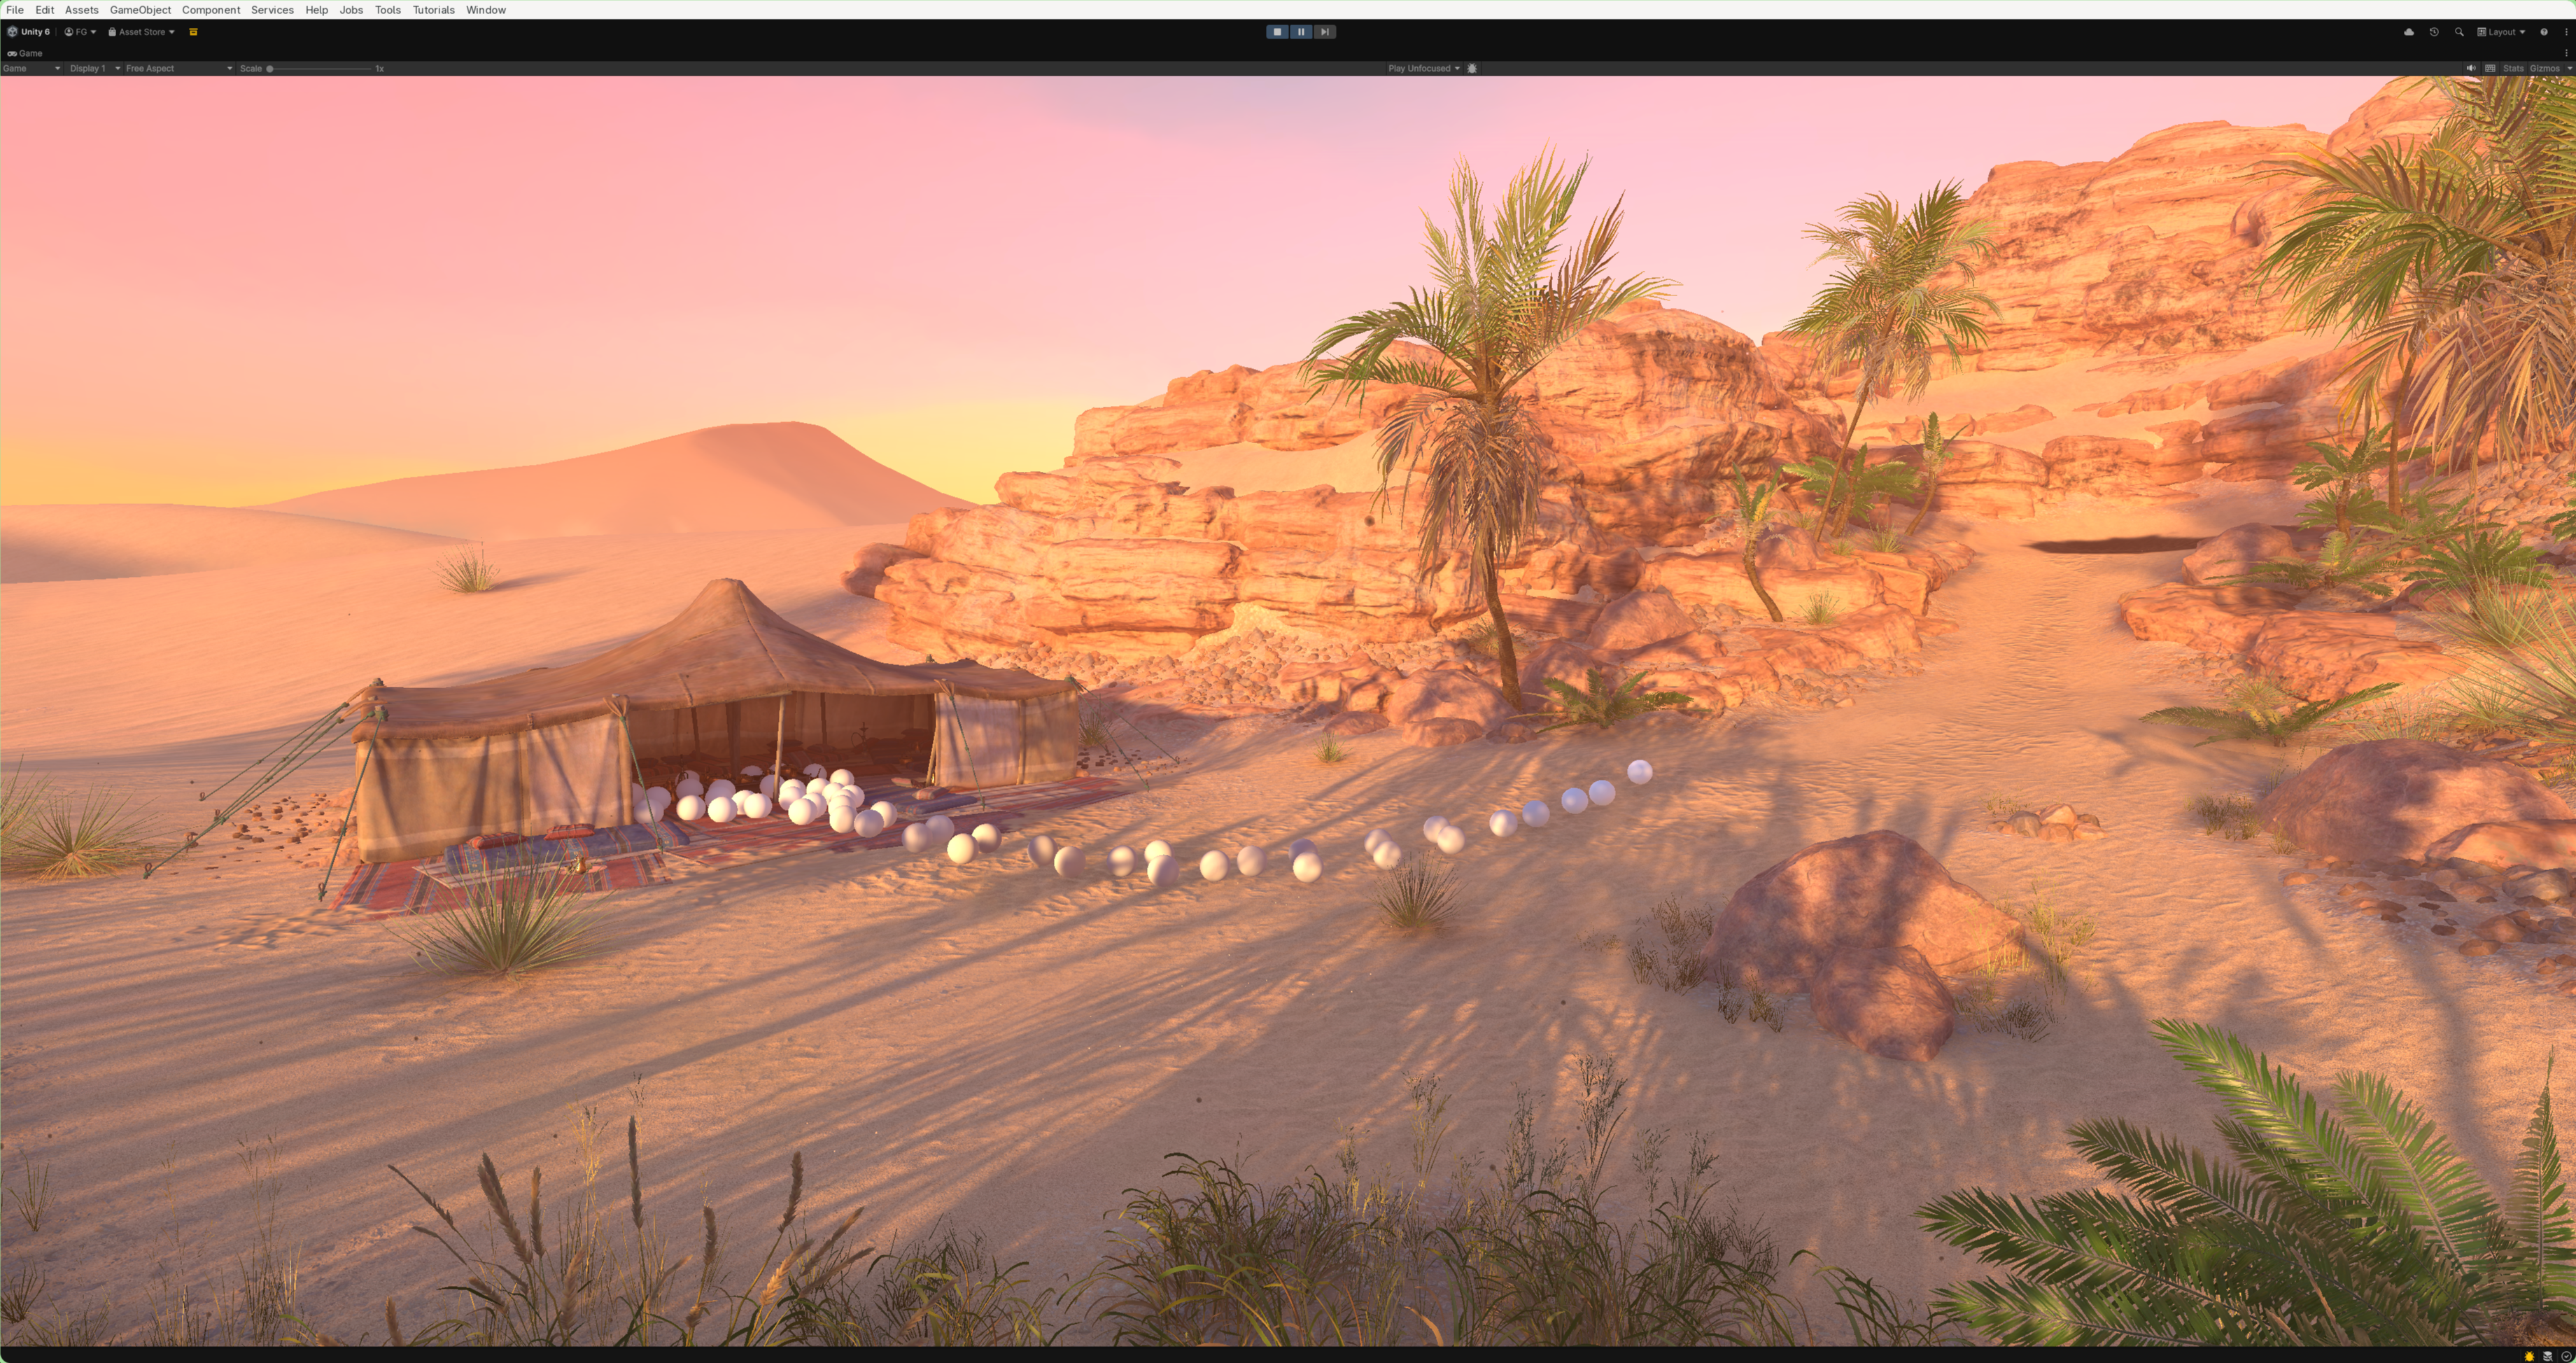
\includegraphics[width=.49\textwidth]{figures/rich-env-7.png}
    \caption{Screenshots of the rich environment scenario with 100 nodes.}\label{fig:rich-env}
\end{figure}
